\documentclass[tikz,border=3pt]{standalone}
\usetikzlibrary{arrows.meta}
\begin{document}
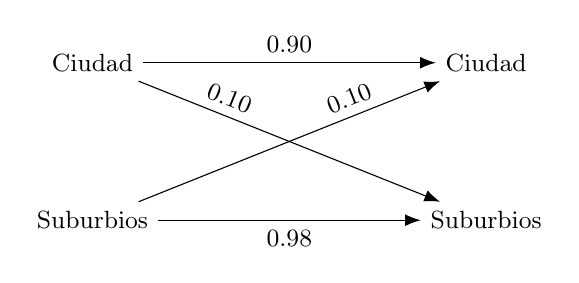
\begin{tikzpicture}[
    node/.style={font=\small},
    lbl/.style={font=\small, midway, sloped, above}
  ]
  \node[node] (c0) at (0,2) {Ciudad};
  \node[node] (s0) at (0,0) {Suburbios};
  \node[node] (c1) at (5,2) {Ciudad};
  \node[node] (s1) at (5,0) {Suburbios};

  \draw[-{Latex[length=2mm]}] (c0) -- node[lbl] {0.90} (c1);
  \draw[-{Latex[length=2mm]}] (c0) -- node[lbl,pos=0.28] {0.10} (s1);
  \draw[-{Latex[length=2mm]}] (s0) -- node[lbl,pos=0.72] {0.10} (c1);
  \draw[-{Latex[length=2mm]}] (s0) -- node[lbl,below] {0.98} (s1);
\end{tikzpicture}
\end{document}
